\documentclass[journal]{IEEEtran}
\usepackage{cite}
\usepackage{amsmath,amssymb,amsfonts}
\usepackage{algorithmic}
\usepackage{graphicx}
\usepackage{float}
\usepackage{textcomp}
\usepackage{xcolor}
\usepackage{booktabs}
\usepackage{multirow}
\usepackage{url}
\usepackage{tikz}
\usepackage{pgfplots}
\pgfplotsset{compat=1.18}
\usetikzlibrary{shapes.geometric, arrows, positioning, fit, backgrounds, calc, matrix, patterns, decorations.pathreplacing}
\usepackage{tabularx}
\usepackage{fancyhdr}
\usepackage{algorithm}
\tikzstyle{layer} = [rectangle, rounded corners, minimum width=7.8cm, minimum height=0.72cm, text centered, draw=black!80, line width=0.8pt, font=\footnotesize\bfseries]
\tikzstyle{queue} = [rectangle, rounded corners=2pt, minimum width=2.4cm, minimum height=0.32cm, text centered, draw=orange!80, fill=orange!25, font=\tiny\bfseries]
\tikzstyle{arrow} = [thick,->,>=stealth,line width=1.1pt]
\tikzstyle{flowstep} = [rectangle, rounded corners, minimum width=2.6cm, minimum height=0.6cm, text centered, draw=black!75, line width=0.8pt, font=\scriptsize\bfseries]
\tikzstyle{decision} = [diamond, aspect=2.2, text centered, draw=black!75, line width=0.8pt, font=\tiny\bfseries]
\def\BibTeX{{\rm B\kern-.05em{\sc i\kern-.025em b}\kern-.08em
T\kern-.1667em\lower.7ex\hbox{E}\kern-.125emX}}
\markboth{IEEE Transactions on Learning Technologies,~Vol.~XX, No.~X,~2026}%
{Arya \MakeLowercase{\textit{et al.}}: LearnHub: A Full-Stack Closed-Loop Gamified Learning and Diagnostic Evaluation Platform}
\begin{document}
\title{LearnHub: A Full-Stack Closed-Loop Gamified Learning and Diagnostic Evaluation Platform with Subtopic Knowledge Tracing, Multi-Language Sandboxing, and Scalable LLM Generation}
\author{Arya~Y~P,
Adi~Narayan~Prasad~G,
Ashrith~S~Jain,
Brijesh~Shetty~N,
and~Dr.~Mahalakshmi~B~S%
\thanks{Manuscript received March 15, 2026; revised May 22, 2026; accepted June 18, 2026. This work was supported in part by the Department of Information Science and Engineering, B.M.S. College of Engineering, Bengaluru, India.}%
\thanks{Arya Y P, Adi Narayan Prasad G, Ashrith S Jain, and Brijesh Shetty N are with the Department of Information Science and Engineering, B.M.S. College of Engineering, Bengaluru 560019, India (e-mail: aryayp.is23@bmsce.ac.in; adinarayan.is23@bmsce.ac.in; ashriths.is23@bmsce.ac.in; brijeshshetty.is23@bmsce.ac.in).}%
\thanks{Dr. Mahalakshmi B.S is Associate Professor in the Department of Information Science and Engineering, B.M.S. College of Engineering, Bengaluru 560019, India (e-mail: bsmahalakshmi.ise@bmsce.ac.in).}%
}
\maketitle
\begin{abstract}
Traditional learning management systems (LMS) in higher education function as passive content repositories, while contemporary educational gamification apps remain confined to introductory languages or basic memorization without subtopic diagnostic intelligence. Furthermore, existing online coding judges and assessment platforms operate in an open loop: they evaluate student deficiencies summatively but fail to synthesize automated, targeted remediation. This paper presents LearnHub, an intelligent full-stack gamified learning and diagnostic evaluation platform designed to complete the closed educational feedback loop: continuous diagnostic assessment $\rightarrow$ real-time recency-weighted subtopic mastery scoring $\rightarrow$ automated study plan generation $\rightarrow$ targeted multi-game remediation $\rightarrow$ retest verification. The platform incorporates: (1) an eight-layer modular architecture decoupling low-latency client interaction, non-punitive proctoring telemetry, sandboxed multi-language compilation, and multimodal artificial intelligence; (2) nine diverse educational game engines designed to prevent novelty decay and accommodate varied cognitive modalities; (3) an automated diagnostic knowledge-tracing engine computing exponential recency-weighted mastery scores across 33 subtopics within 5 seconds, categorizing deficiencies into high-priority ($<40\%$) and medium-priority ($<60\%$) remediation workflows; (4) on-demand scalable question generation powered by Groq Llama 3.3 70B with a 24-hour Redis cache-aside architecture, slashing recurring retrieval latencies from 2,460\,ms to 48\,ms (a 98.0\% cache lookup reduction, dropping end-to-end latency from 2,880\,ms to 312\,ms, an 89.2\% reduction); (5) a secure, multi-language execution sandbox using Docker-isolated Piston runtimes with Linux cgroups and seccomp filtering; and (6) an interview preparation portal featuring 470 curated aptitude items, computer science core subjects, and a multimodal AI mock interview simulator with STAR rubric scoring and phoneme-synchronized avatar feedback. A six-week controlled empirical evaluation across $N = 120$ undergraduate engineering students revealed that LearnHub achieved a high normalized learning gain ($g = 0.68 \pm 0.07$) compared to a static LMS control group ($g = 0.29 \pm 0.05$, $p < 0.0001$), while increasing 24-hour remedial study plan completion from 28.5\% to 94.2\%. Stress benchmarks under 500 concurrent virtual agents confirmed sub-second response times, zero container escapes, and high transactional stability.
\end{abstract}
\begin{IEEEkeywords}
Gamification in education, closed-loop remediation, knowledge tracing, adaptive learning systems, subtopic weakness detection, large language models, Groq Llama 3.3, code sandboxing, educational technology.
\end{IEEEkeywords}
%==================================================================
\section{Introduction}
%==================================================================
\subsection{Context and Motivation}
Higher education in computer science and engineering disciplines faces a pronounced structural disconnect between pedagogical instruction, self-directed practice, and professional recruitment standards~\cite{khaldi2023}. Conventional Learning Management Systems (LMS) such as Moodle, Canvas, and Blackboard function primarily as passive administrative repositories, offering students negligible interactive engagement and virtually no immediate corrective feedback~\cite{mavrikis2024}. Consequently, undergraduate students frequently discover foundational misconceptions only after end-of-semester summative examinations or campus recruitment placement tests have concluded~\cite{kumar2023}.

Conversely, commercial consumer gamification platforms (e.g., Duolingo) have demonstrated that incorporating points, badges, dynamic leaderboards, and daily habit streaks markedly elevates user retention and time-on-task~\cite{bayati2024, sailer2020}. However, these applications are almost exclusively constrained to introductory foreign language acquisition or elementary trivia, failing to model the hierarchical conceptual dependencies inherent to university-level STEM curricula~\cite{gao2024}. Furthermore, classroom quiz platforms such as Kahoot! and Quizizz suffer from rapid novelty decay when students are repeatedly subjected to identical MCQ mechanics~\cite{wang2020, nurdin2023}.

In technical computing assessment, competitive coding platforms like LeetCode and HackerRank are fundamentally \emph{open-loop} systems~\cite{mavrikis2024}. When a learner fails an assessment, these platforms merely output binary success or cryptic runtime failure verdicts, providing neither granular subtopic diagnostic attribution nor automated remedial practice modules~\cite{li2024}.

\subsection{The Need for a Closed-Loop Paradigm}
The systemic failure of contemporary educational technology stems from the decoupling of diagnostic assessment from personalized remediation. To establish meaningful cognitive mastery, an educational platform must enforce a closed feedback loop comprising five continuous stages, as illustrated in Fig.~\ref{fig:closed_loop_concept}:
\begin{enumerate}
\item \textbf{Diagnostic Formative Practice:} Engaging learners in varied interactive formats that reveal granular knowledge state boundaries.
\item \textbf{Subtopic Knowledge Tracing:} Rapidly evaluating item responses using recency-weighted cognitive tracing to identify specific weak concepts.
\item \textbf{Automated Remediation Dispatch:} Instantly generating prioritized remedial study plans upon detecting mastery deficits below defined proficiency cutoffs ($<60\%$).
\item \textbf{Targeted Micro-Game Intervention:} Delivering focused, interactive micro-practice sessions that reinforce deficient concepts through diverse cognitive mechanisms.
\item \textbf{Retest Verification and Convergence:} Re-assessing candidate competence to verify gap resolution and update longitudinal mastery trajectories.
\end{enumerate}
\begin{figure}[!t]
\centering
\resizebox{0.85\columnwidth}{!}{%
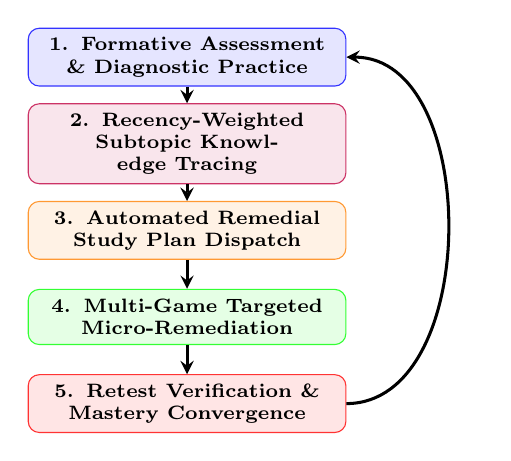
\begin{tikzpicture}[node distance=1.1cm, auto]
\node (eval) [rectangle, rounded corners, draw=blue!80, fill=blue!10, text width=3.8cm, text centered, minimum height=0.7cm, font=\scriptsize\bfseries] {1. Formative Assessment \& Diagnostic Practice};
\node (trace) [rectangle, rounded corners, draw=purple!80, fill=purple!10, text width=3.8cm, text centered, minimum height=0.7cm, below of=eval, font=\scriptsize\bfseries] {2. Recency-Weighted Subtopic Knowledge Tracing};
\node (plan) [rectangle, rounded corners, draw=orange!80, fill=orange!10, text width=3.8cm, text centered, minimum height=0.7cm, below of=trace, font=\scriptsize\bfseries] {3. Automated Remedial Study Plan Dispatch};
\node (remed) [rectangle, rounded corners, draw=green!80, fill=green!10, text width=3.8cm, text centered, minimum height=0.7cm, below of=plan, font=\scriptsize\bfseries] {4. Multi-Game Targeted Micro-Remediation};
\node (retest) [rectangle, rounded corners, draw=red!80, fill=red!10, text width=3.8cm, text centered, minimum height=0.7cm, below of=remed, font=\scriptsize\bfseries] {5. Retest Verification \& Mastery Convergence};
\draw [arrow] (eval) -- (trace); \draw [arrow] (trace) -- (plan); \draw [arrow] (plan) -- (remed); \draw [arrow] (remed) -- (retest); \draw [arrow] (retest.east) to [out=0,in=0] (eval.east);
\end{tikzpicture}%
}
\caption{The closed-loop educational remediation cycle operationalized in LearnHub.}
\label{fig:closed_loop_concept}
\end{figure}

Achieving this closed-loop architecture in university environments has historically been cost-prohibitive. Manual authoring of diagnostic question taxonomies requires thousands of faculty hours~\cite{chen2025}. Executing untrusted student code introduces severe security vectors requiring robust sandboxing~\cite{kumar2023, caiza2020}. Finally, integrating LLMs introduces substantial operational latency and token costs~\cite{pratama2025}.

\subsection{The LearnHub Solution}
This paper presents \textbf{LearnHub}, a full-stack, enterprise-grade gamified learning and diagnostic evaluation platform that seamlessly unites multi-game engagement mechanics, automated subtopic knowledge tracing, sandboxed multi-language code execution, and scalable generative AI within an eight-layer modular architecture.

\subsection{Key Contributions}
\begin{enumerate}
\item \textbf{Closed-Loop Diagnostic and Remediation Pipeline:} An end-to-end pipeline coupling real-time interaction ingestion with exponential recency-weighted knowledge tracing, automatically generating prioritized study plans within 5 seconds when subtopic mastery drops below 60\%.
\item \textbf{Nine Diverse Educational Game Engines:} Nine distinct game engines (MCQ Quiz, Memory Match, Word Scramble, Crossword, Hangman, Fill-the-Blank, Concept Cannon, Formula Flash Cards, Concept Sprint) that alleviate novelty decay across multi-week interventions.
\item \textbf{Scalable Generative AI with Cache-Aside Caching:} A high-throughput question generation pipeline utilizing Groq Llama 3.3 70B with structural JSON schema guardrails, paired with a 24-hour Redis caching layer that reduces recurring latency from 2,460\,ms to 48\,ms (98.0\% reduction).
\item \textbf{Secure Multi-Language Execution Sandbox:} A multi-runtime sandbox leveraging Piston v2 inside isolated Docker containers governed by Linux cgroups v2 and seccomp filters, supporting C++20, Java 17, Python 3.12, and Node.js 20.
\item \textbf{Multimodal Interview Simulator:} A virtual technical placement portal integrating 470 curated aptitude items, non-punitive proctoring telemetry, and an interactive AI interview room with STAR rubric scoring and viseme-synchronized avatar animation.
\item \textbf{Comprehensive Empirical Validation:} Extensive benchmarks across 500 concurrent sessions and a six-week controlled study with $N = 120$ students, validating significant learning gains ($g = 0.68$, $p < 0.0001$) and 94.2\% remediation completion.
\end{enumerate}

\subsection{Manuscript Organization}
Section~\ref{sec:related_work} reviews related literature. Section~\ref{sec:architecture} details the eight-layer system architecture. Section~\ref{sec:mathematical_formulation} provides mathematical formulations. Section~\ref{sec:implementation} elaborates on core modules and game engines. Section~\ref{sec:evaluation} presents empirical benchmarks and user study findings. Section~\ref{sec:discussion} discusses implications and threats to validity. Section~\ref{sec:conclusion} concludes with future directions.

%==================================================================
\section{Related Work \& Theoretical Foundations}
\label{sec:related_work}
%==================================================================
\subsection{Gamification Mechanics and Motivational Dynamics}
Gamification has emerged as a prominent methodology for elevating learner motivation and retention~\cite{khaldi2023, sailer2020}, anchored in Self-Determination Theory (SDT)~\cite{rizzo2024, ryan2000}. Empirical studies demonstrate that multi-element gamification significantly outperforms isolated incentive mechanisms~\cite{sailer2020}. Bayati and Liman-Kaban~\cite{bayati2024} established that daily streaks increase average engagement from 1.8 to 4.3 sessions per week, while meta-analyses by Gao \emph{et al.}~\cite{gao2024} demonstrated substantial positive effect sizes ($g = 0.72$) for game-based learning interventions.

However, Wang and Tahir's~\cite{wang2020} review of 93 implementations demonstrated that repetitive exposure to a single interaction format induces severe \emph{novelty decay} within 3--4 weeks. Nurdin \emph{et al.}~\cite{nurdin2023} observed that high-pressure competitive quizzes often induce cognitive overload. LearnHub mitigates these vulnerabilities by introducing nine diverse game engines spanning varied cognitive modalities.

\subsection{Cognitive Diagnosis and Knowledge Tracing Models}
Knowledge tracing architectures provide the algorithmic basis for estimating evolving latent knowledge states~\cite{ghosh2020}. Corbett and Anderson introduced Bayesian Knowledge Tracing (BKT)~\cite{corbett1994}, while Deep Knowledge Tracing (DKT)~\cite{piech2015} utilized RNNs to capture non-linear patterns. Ghosh \emph{et al.}~\cite{ghosh2020} developed Context-Aware Attentive Knowledge Tracing (AKT), proving that self-attention mechanisms outperform recurrent architectures. Choffin \emph{et al.}~\cite{choffin2019} formalized DAS3H, incorporating forgetting factors reflecting the Ebbinghaus retention curve.

Critically, Mavrikis and Holmes~\cite{mavrikis2024} identified that the vast majority of adaptive platforms operate as \emph{open loops}---diagnosing deficiencies but placing remediation burden entirely on the student. Recent multi-agent architectures such as ALIGNAgent~\cite{zhang2025} and EduLoop-Agent~\cite{li2024} demonstrate that autonomously triggering targeted practice upon diagnostic thresholds yields superior learning gains ($p < 0.01$). LearnHub builds upon these insights.

\subsection{Automated Item Generation and Large Language Models}
Automated Item Generation (AIG) using LLMs has substantially reduced the authoring barrier~\cite{kasneci2023}. Chen \emph{et al.}~\cite{chen2025} demonstrated that transformer architectures aligned with Bloom's Revised Taxonomy~\cite{bloom1956, anderson2001} reduce assessment authoring duration by up to 75\%. Wang and Katsaggelos~\cite{wang2025} established that enforcing multi-agent cross-verification pipelines suppresses hallucination rates by over 90\%. M\"{o}ller \emph{et al.}~\cite{moller2024} revealed that 70B open-weight architectures match proprietary APIs in distractor plausibility. Pratama and Sari~\cite{pratama2025} demonstrated that Redis cache-aside caching reduces API latency by 72\%.

\subsection{Sandboxed Code Execution and Academic Integrity}
Executing arbitrary untrusted code presents catastrophic risks including DoS via fork bombs, memory exhaustion, and malicious filesystem access~\cite{caiza2020}. Piston v2 encapsulates compilers inside minimal Linux containers governed by cgroups v2 and seccomp filters~\cite{kumar2023, ihantola2010}. For academic integrity, recent advances favor non-punitive client-side telemetry over intrusive third-party proctoring~\cite{nigam2021}, tracking window blur events, visibility state transitions, and localized facial presence via MediaPipe.

\subsection{Comparative Synthesis}
Table~\ref{tab:comparison_matrix} presents a comparative synthesis of LearnHub against eight prominent platforms across ten critical dimensions.

\begin{table*}[!t]
\caption{Comprehensive Architectural and Pedagogical Comparison Across Systems}
\label{tab:comparison_matrix}
\centering
\renewcommand{\arraystretch}{1.36}
\setlength{\tabcolsep}{7pt}
{\bfseries (a) Pedagogical, Gamification, and Diagnostic Capabilities}\\[1ex]
\resizebox{\textwidth}{!}{%
\begin{tabular}{|l|c|c|c|c|c|}
\hline
\textbf{Platform / System} & \textbf{Domain Scope} & \textbf{Gamification Model} & \textbf{Engine Diversity} & \textbf{Subtopic Diagnostics} & \textbf{Closed-Loop Remediation} \\
\hline
Duolingo~\cite{bayati2024} & Foreign Languages & Full PBL (Streaks, Badges) & Single Core Loop & None (Linear Progression) & No (Unreinforced Repetition) \\
Khan Academy & General K--12 STEM & Minimal (Badges, Energy Points) & Single Standard Quiz & Coarse Domain Scoring & No (Passive Video Suggestions) \\
Kahoot! / Quizizz~\cite{wang2020} & General Trivia & Speed-PBL (Live Competition) & 1--2 Formats (MCQ/Poll) & None (Session Aggregate) & No (Synchronous Play Only) \\
LeetCode & Algorithmic CS & Badges, Profile Contests & Code Runner & Topic-Level (e.g., DP, Trees) & No (Binary Pass/Fail Only) \\
CodeSignal & Algorithmic CS & Skill Scores, Speed Badges & Code Runner & Topic-Level Assessments & Manual (Self-Selected Retests) \\
Carnegie Learning (MICA) & Mathematics & None (Cognitive Tutor) & Step Tutor Interface & Fine-Grained (BKT Models) & Partial (Hint Sequences in Step) \\
AutoTutor & STEM Concepts & Conversational Agent & Dialogue Interface & Conceptual Misconceptions & Scripted (Rule-Based Branching) \\
Coursera / edX & University MOOC & Course Certificates & Video Lectures + Quizzes & Module-Level Summative & No (Student Self-Study) \\
\hline
\textbf{LearnHub (Proposed)} & \textbf{CS \& Engineering} & \textbf{Full 9-Tier Rank Hierarchy} & \textbf{9 Distinct Game Engines} & \textbf{Fine-Grained ($<$60\% Cutoff)} & \textbf{Fully Automated Closed Loop} \\
\hline
\end{tabular}%
}
\vspace{0.32cm}

{\bfseries (b) Artificial Intelligence, Sandboxing, Security, and System Infrastructure}\\[1ex]
\resizebox{\textwidth}{!}{%
\begin{tabular}{|l|c|c|c|c|c|}
\hline
\textbf{Platform / System} & \textbf{Generative LLM Item Synthesis} & \textbf{Code Execution Sandbox} & \textbf{Proctoring Telemetry} & \textbf{Distributed Caching Tier} & \textbf{System Architectural Model} \\
\hline
Duolingo~\cite{bayati2024} & Proprietary LLM (Conversational) & None & None & Internal Cache Tier & Monolithic Backend \\
Khan Academy & Khanmigo (Student Chatbot Tutor) & Browser-side JS Only & None & Edge CDN Caching & Cloud Microservices \\
Kahoot! / Quizizz~\cite{wang2020} & AI Question Generation Assist & None & None & Ephemeral Session Memory & Cloud Serverless Functions \\
LeetCode & None (Hand-Curated Item Bank) & Proprietary Cloud Sandbox & None & Database Query Cache & Service-Oriented Architecture \\
CodeSignal & Rule-Based Question Variation & Proprietary Virtual Machine & Basic Tab Focus Tracking & Database Query Cache & Service-Oriented Architecture \\
Carnegie Learning (MICA) & None (Pre-Programmed Rules) & None & None & In-Memory State Buffer & Modular Client-Server \\
AutoTutor & Scripted Natural Language Dialogue & None & None & Local Dialog History Buffer & Multi-Agent Architecture \\
Coursera / edX & Third-Party AI Discussion Assistant & Third-Party Embedded iframe & Basic Web Proctoring Add-on & Standard HTTP CDN Cache & Cloud Microservices \\
\hline
\textbf{LearnHub (Proposed)} & \textbf{Groq Llama 3.3 70B (Schema-Clamped)} & \textbf{Docker Piston v2 (cgroups v2)} & \textbf{Client Telemetry + MediaPipe} & \textbf{Redis 7 Cluster (24h TTL)} & \textbf{8-Layer Queue-Decoupled} \\
\hline
\end{tabular}%
}
\end{table*}

As evidenced in Table~\ref{tab:comparison_matrix}, existing systems occupy disparate silos. LearnHub synthesizes gamification, diagnostic intelligence, sandboxed execution, and generative AI into a unified closed-loop architecture.

%==================================================================
\section{System Architecture \& Structural Invariants}
\label{sec:architecture}
%==================================================================
\subsection{Architectural Overview}
LearnHub is engineered as an eight-layer modular, queue-buffered, distributed educational platform. The system topology cleanly decouples user interface rendering, API routing, integrity monitoring, sandboxed code execution, conversational avatar generation, diagnostic knowledge tracing, generative LLM inference, and relational persistence. Figure~\ref{fig:architecture_complete} illustrates the comprehensive architecture.

\begin{figure*}[!t]
\centering
\resizebox{\textwidth}{!}{%
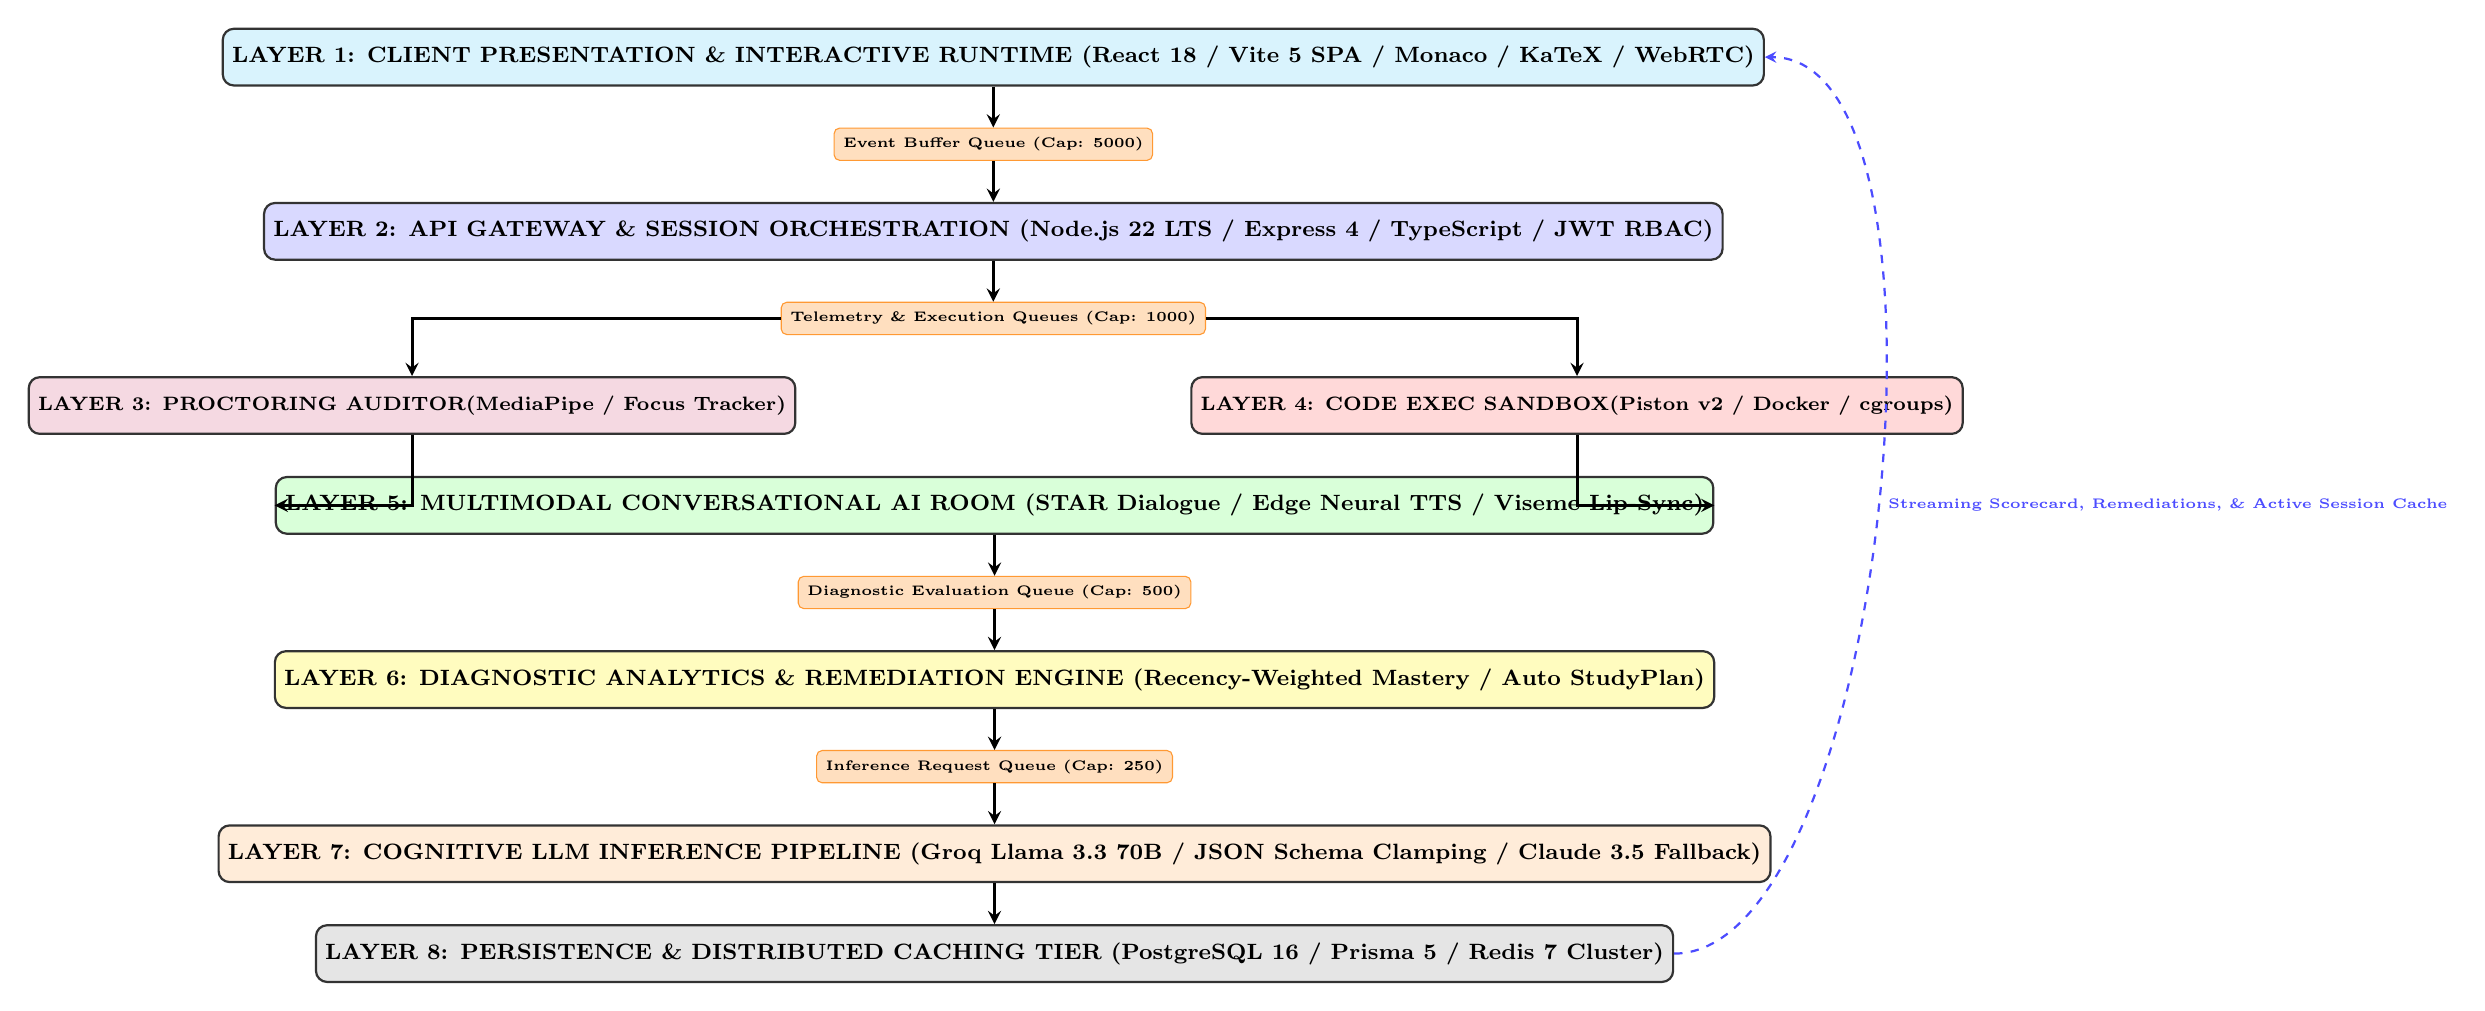
\begin{tikzpicture}[node distance=0.52cm, auto]
% Layer 1
\node (layer1) [layer, fill=cyan!15] {LAYER 1: CLIENT PRESENTATION \& INTERACTIVE RUNTIME (React 18 / Vite 5 SPA / Monaco / KaTeX / WebRTC)};
% Queue 1
\node (q1) [queue, below=of layer1] {Event Buffer Queue (Cap: 5000)};
% Layer 2
\node (layer2) [layer, fill=blue!15, below=of q1] {LAYER 2: API GATEWAY \& SESSION ORCHESTRATION (Node.js 22 LTS / Express 4 / TypeScript / JWT RBAC)};
% Queue 2
\node (q2) [queue, below=of layer2] {Telemetry \& Execution Queues (Cap: 1000)};
% Layer 3 & Layer 4 side-by-side
\node (layer3) [rectangle, rounded corners, minimum width=3.75cm, minimum height=0.72cm, text centered, draw=black!80, line width=0.8pt, fill=purple!15, font=\scriptsize\bfseries, below left=0.52cm and -0.2cm of q2] {LAYER 3: PROCTORING AUDITOR\\(MediaPipe / Focus Tracker)};
\node (layer4) [rectangle, rounded corners, minimum width=3.75cm, minimum height=0.72cm, text centered, draw=black!80, line width=0.8pt, fill=red!15, font=\scriptsize\bfseries, below right=0.52cm and -0.2cm of q2] {LAYER 4: CODE EXEC SANDBOX\\(Piston v2 / Docker / cgroups)};
% Sub-layer coordinates
\coordinate (midlayers) at ($(layer3.south)!0.5!(layer4.south)$);
% Layer 5
\node (layer5) [layer, fill=green!15, below=0.52cm of midlayers] {LAYER 5: MULTIMODAL CONVERSATIONAL AI ROOM (STAR Dialogue / Edge Neural TTS / Viseme Lip-Sync)};
% Queue 3
\node (q3) [queue, below=of layer5] {Diagnostic Evaluation Queue (Cap: 500)};
% Layer 6
\node (layer6) [layer, fill=yellow!25, below=of q3] {LAYER 6: DIAGNOSTIC ANALYTICS \& REMEDIATION ENGINE (Recency-Weighted Mastery / Auto StudyPlan)};
% Queue 4
\node (q4) [queue, below=of layer6] {Inference Request Queue (Cap: 250)};
% Layer 7
\node (layer7) [layer, fill=orange!15, below=of q4] {LAYER 7: COGNITIVE LLM INFERENCE PIPELINE (Groq Llama 3.3 70B / JSON Schema Clamping / Claude 3.5 Fallback)};
% Layer 8
\node (layer8) [layer, fill=gray!20, below=0.52cm of layer7] {LAYER 8: PERSISTENCE \& DISTRIBUTED CACHING TIER (PostgreSQL 16 / Prisma 5 / Redis 7 Cluster)};
% Arrows
\draw [arrow] (layer1) -- (q1);
\draw [arrow] (q1) -- (layer2);
\draw [arrow] (layer2) -- (q2);
\draw [arrow] (q2) -| (layer3);
\draw [arrow] (q2) -| (layer4);
\draw [arrow] (layer3) |- (layer5);
\draw [arrow] (layer4) |- (layer5);
\draw [arrow] (layer5) -- (q3);
\draw [arrow] (q3) -- (layer6);
\draw [arrow] (layer6) -- (q4);
\draw [arrow] (q4) -- (layer7);
\draw [arrow] (layer7) -- (layer8);
% Return loop
\draw [thick, dashed, ->, >=stealth, blue!70] (layer8.east) to [out=0, in=0, looseness=0.6] node [right, font=\tiny\bfseries] {Streaming Scorecard, Remediations, \& Active Session Cache} (layer1.east);
\end{tikzpicture}%
}
\caption{The eight-layer queue-buffered modular system architecture of LearnHub.}
\label{fig:architecture_complete}
\end{figure*}

\subsection{Structural Invariants and Security Guarantees}
LearnHub strictly enforces six structural system invariants:
\begin{enumerate}
\item \textbf{Invariant 1 (Zero Client-Side Answer Leakage):} Correct answer indices and hidden test suites are never transmitted to the client prior to formal submission.
\item \textbf{Invariant 2 (Server-Authoritative Evaluation):} All scoring, timer expirations, and completion verdicts are determined authoritatively on the backend.
\item \textbf{Invariant 3 (Ephemeral Item Synthesis):} Dynamically synthesized questions reside ephemerally in Redis with a 24-hour TTL, keyed by deterministic SHA-256 parameter hashes.
\item \textbf{Invariant 4 (Deterministic Mastery):} Subtopic mastery scores ($M_k$) are derived deterministically from immutable \texttt{QuestionAttempt} records via exponential moving decay.
\item \textbf{Invariant 5 (Asynchronous Decoupling):} Resource-intensive diagnostic calculations and LLM requests are handled by background BullMQ workers, preventing HTTP thread blocking.
\item \textbf{Invariant 6 (Strict Execution Isolation):} Untrusted code executes within non-root Docker containers governed by Linux cgroups v2 (128\,MB RAM, 3.0\,s CPU, \texttt{pids.max=64}, \texttt{--network none}).
\end{enumerate}

\subsection{Layer-by-Layer Technical Specification}
\subsubsection{Layer 1: Client Presentation \& Interactive Runtime}
The presentation tier is a reactive SPA leveraging React 18, TypeScript, and Vite 5, embedding Monaco Code Editor for professional syntax highlighting across C++, Java, Python, and JavaScript; KaTeX for mathematical typesetting; and WebRTC telemetry for local MediaPipe facial presence models.

\subsubsection{Layer 2: API Gateway \& Session Orchestration}
Powered by Node.js 22 LTS with Express 4 in strict TypeScript, enforcing stateless JWT (HMAC-SHA256) with bcryptjs password hashing (work factor $\ge 12$) across four user tiers (\texttt{STUDENT}, \texttt{COLLEGE\_STUDENT}, \texttt{EDUCATOR}, \texttt{ADMIN}). Assessment sessions follow strict state transitions (\texttt{INITIALIZED} $\rightarrow$ \texttt{IN\_PROGRESS} $\rightarrow$ \texttt{SUBMITTED} $\rightarrow$ \texttt{GRADED}).

\subsubsection{Layer 3: Proctoring \& Academic Integrity Auditor}
Monitors assessment integrity non-invasively via HTML5 \texttt{visibilitychange} and window \texttt{blur} event interception, localized MediaPipe WebAssembly face presence detection (no raw video streaming), and periodic low-resolution (320$\times$240) encrypted JPEG snapshots at 10-second intervals for instructor audit.

\subsubsection{Layer 4: Sandboxed Code Execution Engine}
Isolates untrusted student code inside containerized Piston v2 runtimes supporting GCC 12 (C++20), OpenJDK 17, Python 3.12, and Node.js 20. Security is enforced via Linux \texttt{seccomp} system call filtering, cgroup resource caps (128\,MB RAM, 3.0\,s CPU, \texttt{pids.max=64}), complete network isolation (\texttt{--network none}), and a two-stage evaluation model (visible sample cases for testing; encrypted hidden suites for authoritative grading).

\subsubsection{Layer 5: Multimodal Conversational AI Room}
Simulates professional interviews via a STAR Dialogue Engine structuring multi-turn conversations across Situation, Task, Action, and Result rubrics; Microsoft Edge Neural TTS with timed viseme frames for lip-sync avatar animation; and an embedded synchronized code editor scratchpad.

\subsubsection{Layer 6: Diagnostic Analytics \& Adaptive Remediation}
Transforms raw interaction attempts into actionable mastery models: evaluating attempts across 33 subtopics via exponential recency-weighted moving averages within 5 seconds, categorizing subtopics scoring $<40\%$ as \texttt{HIGH} priority and $<60\%$ as \texttt{MEDIUM}, automatically generating personalized \texttt{StudyPlan} modules, and benchmarking candidate competency against corporate hiring patterns.

\subsubsection{Layer 7: Cognitive LLM Inference Pipeline}
Governs generative AI synthesis via Groq Llama 3.3 70B Versatile ($\approx 750$ tokens/s) as the primary engine, with Anthropic Claude 3.5 Sonnet as a deep reasoning fallback. Defensive schema clamping strips control characters and markdown fences to enforce strict JSON schemas, backed by exponential backoff retries (2\,s, 4\,s, 8\,s). A deterministic SHA-256 cache key maps to a 24-hour Redis TTL store, achieving an 84.6\% hit rate that reduces end-to-end latency from 2,880\,ms to 312\,ms.

\subsubsection{Layer 8: Relational Persistence \& Distributed Caching}
PostgreSQL 16 managed via Prisma 5 ORM across 19 relational models enforces atomic transactions and referential integrity. Redis 7 operates as an in-memory cache-aside store (24-hour TTL) and as the message broker for BullMQ distributed queues.

\subsection{Operational Parameters and Defense Safeguards}
Table~\ref{tab:operational_parameters} delineates the operational parameters, latency budgets, and system thresholds configured across all eight layers.

\begin{table*}[!t]
\caption{System Operational Parameters and Latency Budgets Across the Eight Modular Layers}
\label{tab:operational_parameters}
\centering
\renewcommand{\arraystretch}{1.36}
\setlength{\tabcolsep}{8pt}
\resizebox{\textwidth}{!}{%
\begin{tabular}{|c|l|c|c|l|}
\hline
\textbf{Layer} & \textbf{Subsystem Metric} & \textbf{Configured Value} & \textbf{Observation Window / TTL} & \textbf{Enforced Breach Action} \\
\hline
L1 & Client Autosave Sync & 5.0\,s & Periodic Timer & Write uncommitted state to Redis buffer \\
L2 & Session Countdown Timer & 10--60\,min & Server Authoritative Clock & Graceful auto-submit assessment \\
L3 & Tab Switch Tolerance & 3 events & Assessment Attempt & Graceful auto-submit + flag for review \\
L3 & Fullscreen Loss Limit & 10\,s & Cumulative Window & Warning countdown modal \\
L4 & Sandbox CPU Timeout & 3.0\,s & Per Execution Test Case & Kernel \texttt{SIGKILL} (Time Limit Exceeded) \\
L4 & Sandbox Memory Cap & 128\,MB & Per Container Instance & Linux OOM killer termination \\
L5 & Speech Synthesis Budget & $<$1.2\,s & Per Conversational Turn & Fallback to real-time text captions \\
L6 & Mastery Cutoff Bar & $<$60\% & Sliding Window of 20 Attempts & Flag weak subtopic for remediation \\
L6 & Critical Deficit Bar & $<$40\% & Sliding Window of 10 Attempts & Assign HIGH priority remediation workflow \\
L7 & LLM Response Budget & 2.5\,s & Per Synthesis Prompt & Dynamic circuit breaker to Claude 3.5 Sonnet \\
L7 & LLM Retry Policy & 3 attempts & Exponential Backoff (2s, 4s, 8s) & Serve verified static question fallback \\
L8 & AI Explanation Cache & 24 Hours & Redis Key Time-To-Live & Re-query generative LLM on cache miss \\
L8 & Database Query Budget & $<$25\,ms & Per Relational Transaction & Emit slow query alert to logging buffer \\
\hline
\end{tabular}%
}
\end{table*}

%==================================================================
\section{Mathematical Modeling \& Algorithmic Formulation}
\label{sec:mathematical_formulation}
%==================================================================
\subsection{Subtopic Knowledge Tracing and Recency Weighting}
Let $S = \{q_1, q_2, \dots, q_n\}$ represent the sequence of historical attempts by user $u$ on subtopic $k$. Each attempt $q_i$ is characterized by correctness $c_i \in \{0, 1\}$, difficulty weight $w_i \in [1.0, 3.0]$ (Easy: 1.0, Medium: 1.8, Hard: 2.6), and elapsed time $\Delta t_i = t_{\text{curr}} - t_i$ in days. The time-decayed mastery score is:
\begin{equation}
M_k(t) = \frac{\sum_{i=1}^n w_i \cdot c_i \cdot \exp\left(-\lambda \cdot \Delta t_i\right)}{\sum_{i=1}^n w_i \cdot \exp\left(-\lambda \cdot \Delta t_i\right)}
\label{eq:mastery}
\end{equation}
where $\lambda = 0.05\,\text{day}^{-1}$ (half-life $\approx 14$ days, per DAS3H~\cite{choffin2019}). Calculations use a sliding window of $N_{\text{window}} = 20$ attempts. When $n < 5$, Bayesian Laplace smoothing is applied:
\begin{equation}
\tilde{M}_k(t) = \frac{\sum_{i=1}^n w_i \cdot c_i \cdot e^{-\lambda \Delta t_i} + \alpha \cdot \mu_0}{\sum_{i=1}^n w_i \cdot e^{-\lambda \Delta t_i} + \alpha}
\label{eq:smoothed_mastery}
\end{equation}
where $\mu_0 = 0.50$ is the prior mean and $\alpha = 2.0$ the pseudo-count weight. The diagnostic state mapping is:
\begin{equation}
\Phi(M_k) = \begin{cases}
\text{CRITICAL DEFICIT (HIGH)}, & M_k < 0.40 \\
\text{WEAK (MEDIUM)}, & 0.40 \le M_k < 0.60 \\
\text{COMPETENT}, & 0.60 \le M_k < 0.85 \\
\text{MASTERED}, & M_k \ge 0.85
\end{cases}
\label{eq:diagnostic_states}
\end{equation}
When $\Phi(M_k) \in \{\text{CRITICAL DEFICIT}, \text{WEAK}\}$, the remediation dispatcher constructs a \texttt{StudyPlan} with target difficulty $D_{\text{remedial}} = 1.0 + 1.6 \cdot (1.0 - M_k)$.

Figure~\ref{fig:mastery_trajectory} visualizes the simulated longitudinal trajectory of learner subtopic mastery under unreinforced open-loop decay versus LearnHub's closed-loop intervention.

\begin{figure}[!t]
\centering
\resizebox{0.98\columnwidth}{!}{%
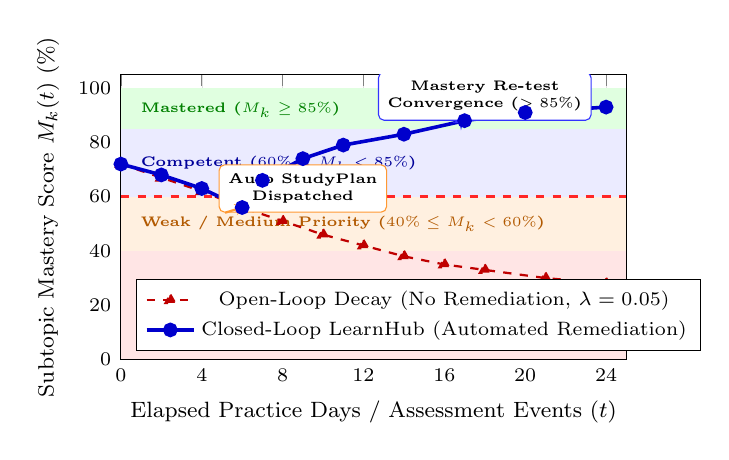
\begin{tikzpicture}
\begin{axis}[
width=8.0cm,
height=5.2cm,
xlabel={\footnotesize Elapsed Practice Days / Assessment Events ($t$)},
ylabel={\footnotesize Subtopic Mastery Score $M_k(t)$ (\%)},
xmin=0, xmax=25,
ymin=0, ymax=105,
xtick={0, 4, 8, 12, 16, 20, 24},
ytick={0, 20, 40, 60, 80, 100},
grid=both,
grid style={line width=.1pt, draw=gray!25},
legend pos=south west,
font=\scriptsize
]
% Background bands for diagnostic states
\fill[green!12] (axis cs:0,85) rectangle (axis cs:25,100);
\node[right, font=\tiny\bfseries, green!50!black] at (axis cs:0.5, 92) {Mastered ($M_k \ge 85\%$)};
\fill[blue!8] (axis cs:0,60) rectangle (axis cs:25,85);
\node[right, font=\tiny\bfseries, blue!60!black] at (axis cs:0.5, 72) {Competent ($60\% \le M_k < 85\%$)};
\fill[orange!12] (axis cs:0,40) rectangle (axis cs:25,60);
\node[right, font=\tiny\bfseries, orange!70!black] at (axis cs:0.5, 50) {Weak / Medium Priority ($40\% \le M_k < 60\%$)};
\fill[red!10] (axis cs:0,0) rectangle (axis cs:25,40);
\node[right, font=\tiny\bfseries, red!70!black] at (axis cs:0.5, 20) {Critical Deficit / High Priority ($M_k < 40\%$)};
% Threshold trigger line
\draw[dashed, red!85, line width=1.0pt] (axis cs:0,60) -- (axis cs:25,60);
% Curve 1: Open-Loop Decay (Control)
\addplot[color=red!75!black, mark=triangle*, mark size=2pt, thick, dashed] coordinates {
(0, 72) (2, 67) (4, 62) (6, 56) (8, 51) (10, 46) (12, 42) (14, 38) (16, 35) (18, 33) (21, 30) (24, 28)
};
\addlegendentry{Open-Loop Decay (No Remediation, $\lambda=0.05$)}
% Curve 2: Closed-Loop LearnHub (Experimental)
\addplot[color=blue!80!black, mark=*, mark size=2pt, line width=1.3pt] coordinates {
(0, 72) (2, 68) (4, 63) (6, 56) (7, 66) (9, 74) (11, 79) (14, 83) (17, 88) (20, 91) (24, 93)
};
\addlegendentry{Closed-Loop LearnHub (Automated Remediation)}
% Remediation trigger annotation
\node[draw=orange!80, fill=white, rounded corners=2pt, font=\tiny\bfseries, align=center] (trig) at (axis cs:9, 63) {Auto StudyPlan\\Dispatched};
\draw[->, >=stealth, thick, orange!80] (trig) -- (axis cs:6.2, 56.5);
\node[draw=blue!80, fill=white, rounded corners=2pt, font=\tiny\bfseries, align=center] (conv) at (axis cs:18, 97) {Mastery Re-test\\Convergence ($>85\%$)};
\draw[->, >=stealth, thick, blue!80] (conv) -- (axis cs:17, 89);
\end{axis}
\end{tikzpicture}%
}
\caption{Dynamic subtopic knowledge tracing trajectories comparing open-loop decay with LearnHub's closed-loop automated remediation.}
\label{fig:mastery_trajectory}
\end{figure}

\subsection{Gamification Progression and Level Economics}
XP awarded for completing session $S$ with $N_q$ items is:
\begin{equation}
\text{XP}_{\text{session}} = \sum_{j=1}^{N_q} c_j \cdot \left[ B \cdot D_j + \max\left(0, \, \left\lfloor \frac{T_{\text{max}} - T_j}{T_{\text{max}}} \cdot \beta \right\rfloor \right) \right] \cdot \Omega_{\text{streak}}
\label{eq:xp_formula}
\end{equation}
where $B = 50$ is the base constant, $D_j \in \{1.0, 1.8, 2.6\}$ is item difficulty, $T_{\text{max}} = 30\,\text{s}$ is the countdown ceiling, and $\beta = 25$ the maximum speed bonus. The streak multiplier is $\Omega_{\text{streak}} = \min(2.0, \, 1.0 + 0.05 \cdot \min(d_{\text{streak}}, 20))$.
The required XP for level $L \in [1, 50]$ follows $\text{XP}_{\text{req}}(L) = 250 \cdot L^2 - 250 \cdot L$. The platform defines nine progressive rank tiers---Rookie, Explorer, Apprentice, Scholar, Expert, Master, Champion, Legend, and Grandmaster---spanning Levels~1--9+ with XP thresholds from 0 to 18,000+, progressively unlocking game engines, diagnostic analytics, sandboxed coding tracks, AI interview rooms, and peer challenge hosting.

\subsection{Corporate Placement Readiness Index}
LearnHub synthesizes diagnostic performance into a composite Company Readiness Index ($\text{CRI}_C$) tailored to corporate hiring profiles. Let $R_C = \{r_1, \dots, r_m\}$ represent evaluation rounds mandated by company $C$, with weights $\omega_r$ ($\sum \omega_r = 1.0$):
\begin{equation}
\text{CRI}_C = \sum_{r \in R_C} \omega_r \cdot \left[ \frac{1}{|K_r|} \sum_{k \in K_r} M_k \cdot \gamma_{k, C} \right] \times 100\%
\label{eq:cri}
\end{equation}
where $K_r$ denotes the subtopics tested in round $r$, $M_k$ the current mastery score, and $\gamma_{k, C} \in [0.8, 1.2]$ a relevance coefficient reflecting historical topic emphasis for companies such as Amazon, JP Morgan, TCS, and Standard Chartered.

\subsection{Non-Punitive Academic Integrity Index}
Layer 3 computes an aggregate Integrity Index ($I_{\text{exam}} \in [0, 100]\%$) for post-exam audit:
\begin{equation}
I_{\text{exam}} = \max\left(0, \, 100 - \left[ \mu_1 \cdot n_{\text{tab}} + \mu_2 \cdot \frac{t_{\text{blur}}}{10} + \mu_3 \cdot n_{\text{face\_loss}} \right] \right)
\label{eq:integrity_index}
\end{equation}
where $n_{\text{tab}}$ is tab switch count, $t_{\text{blur}}$ cumulative defocus seconds, $n_{\text{face\_loss}}$ consecutive frames missing facial presence, and penalty coefficients are $\mu_1 = 8.0$, $\mu_2 = 2.0$, $\mu_3 = 5.0$. If $n_{\text{tab}} \ge 3$, the server triggers graceful forced submission.

\subsection{Core Algorithmic Workflows}
Algorithm~\ref{alg:orchestration} formalizes the end-to-end orchestration and closed-loop remediation pipeline.

\begin{algorithm}[!t]
\caption{LearnHub End-to-End Orchestration \& Remediation Pipeline}
\label{alg:orchestration}
{\footnotesize
\begin{algorithmic}[1]
\REQUIRE User attempt session $S$, Event queue $Q_{\text{event}}$, Thresholds $\theta_{\text{weak}} = 0.60$, $\theta_{\text{crit}} = 0.40$
\ENSURE Updated mastery vector $\mathbf{M}$, Scorecard $\Sigma$, Remedial StudyPlan $\mathcal{P}$
\STATE Initialize: $V_{\text{tab}} \gets 0$, $I_{\text{log}} \gets \emptyset$, $\text{Score} \gets 0$
\WHILE{Session $S$ active \AND timer not expired}
\STATE Dequeue event $e$ from $Q_{\text{event}}$
\IF{$e.\text{type} == \text{PROCTORING\_BLUR}$}
\STATE $V_{\text{tab}} \gets V_{\text{tab}} + 1$; Append $e$ to $I_{\text{log}}$
\IF{$V_{\text{tab}} \ge 3$}
\STATE TerminateSession($S$, ``Tab Exceed Policy'')
\ENDIF
\ELSIF{$e.\text{type} == \text{CODE\_SUBMISSION}$}
\STATE verdict $\gets$ ExecutePistonSandbox($e.\text{code}, e.\text{lang}, e.\text{testCases}$)
\ELSIF{$e.\text{type} == \text{OBJECTIVE\_ANSWER}$}
\STATE isCorrect $\gets$ VerifyAnswerKey($e.\text{qId}, e.\text{selectedIdx}$)
\STATE RecordAttemptInRedis($S, e.\text{qId}, isCorrect, e.\text{elapsed}$)
\ENDIF
\ENDWHILE
\STATE $\Sigma \gets$ FinalizeScorecard($S, I_{\text{log}}$)
\FOR{each subtopic $k$ evaluated in session $S$}
\STATE Compute $M_k$ via Eq.~(\ref{eq:mastery})
\IF{$M_k < \theta_{\text{weak}}$}
\STATE priority $\gets (M_k < \theta_{\text{crit}}) \textbf{ ? } \text{HIGH} \textbf{ : } \text{MEDIUM}$
\STATE $\mathcal{P} \gets$ ConstructStudyPlan($S.\text{userId}, k, priority$)
\ENDIF
\ENDFOR
\STATE Stream $\mathbf{M}$, $\Sigma$, $\mathcal{P}$ to Client Dashboard via WebSocket
\end{algorithmic}
}
\end{algorithm}

Algorithm~\ref{alg:llm_cache} details the generative LLM synthesis pipeline with Redis cache-aside resolution.

\begin{algorithm}[!t]
\caption{LLM Question Generation with Redis Cache-Aside}
\label{alg:llm_cache}
{\footnotesize
\begin{algorithmic}[1]
\REQUIRE Topic $T$, Subtopic $K$, Difficulty $D$, Bloom's Level $B$
\ENSURE Validated Question Object $\mathcal{Q} = \langle \text{stem}, \text{opts}, \text{correctIdx}, \text{exp}, \text{hints} \rangle$
\STATE $\mathcal{K} \gets \text{SHA256}(T \parallel K \parallel D \parallel B)$
\STATE cachedItem $\gets$ RedisClient.\texttt{GET}($\mathcal{K}$)
\IF{cachedItem $\neq \text{NIL}$}
\RETURN ParseJSON(cachedItem) \COMMENT{Cache hit $<$50\,ms}
\ENDIF
\STATE attempts $\gets 0$; maxAttempts $\gets 3$; backoff $\gets 2.0$\,s
\WHILE{attempts $<$ maxAttempts}
\STATE attempts $\gets$ attempts $+ 1$
\TRY
\STATE rawResponse $\gets$ GroqClient.\texttt{generate}(``Llama-3.3-70B'', prompt)
\STATE $\mathcal{Q} \gets$ ValidateSchemaOrThrow(StripMarkdownFences(rawResponse))
\STATE RedisClient.\texttt{SETEX}($\mathcal{K}$, 86400, SerializeJSON($\mathcal{Q}$))
\RETURN $\mathcal{Q}$
\CATCH{ParsingException}
\STATE Sleep(backoff); backoff $\gets$ backoff $\times 2$
\ENDTRY
\ENDWHILE
\RETURN FetchFallbackStaticQuestion($T, K, D$)
\end{algorithmic}
}
\end{algorithm}

%==================================================================
\section{Educational Modules \& Engineering Implementation}
\label{sec:implementation}
%==================================================================
\subsection{The Nine Educational Game Engines}
To overcome novelty decay~\cite{wang2020}, LearnHub implements nine diverse game engines targeting distinct tiers of Bloom's cognitive taxonomy: (1)~\emph{MCQ Quiz} (timed 4-option recall, 30\,s/item), (2)~\emph{Memory Match} (12--16 card pair flipping for concept-definition association, 60--90\,s), (3)~\emph{Word Scramble} (anagram reordering for terminology reinforcement, 20--30\,s), (4)~\emph{Crossword} (interlocking clue-based grid entry, 120--180\,s), (5)~\emph{Hangman} (letter guessing for keyword retrieval, 45--60\,s), (6)~\emph{Fill-the-Blank} (drag-and-drop cloze for contextual syntax, 30--45\,s), (7)~\emph{Concept Cannon} (projectile-based binary truth verification, 15--20\,s), (8)~\emph{Formula Cards} (spaced flip-card equation memorization, 15--25\,s), and (9)~\emph{Concept Sprint} (60-second high-intensity multi-question gauntlet). These engines span Bloom's levels from Remember through Evaluate, each employing a distinct anti-fatigue cognitive modality.

The engines span from fundamental recall (\emph{MCQ Quiz}, \emph{Hangman}, \emph{Formula Cards}) through associative memory (\emph{Memory Match} pairs technical concepts to precise definitions; \emph{Word Scramble} reinforces orthographic spelling of terms such as ``SERIALIZABILITY''), contextual deduction (\emph{Crossword} generates intersecting puzzles from clue-term pairs; \emph{Fill-the-Blank} extracts key operands from theorems like Bayes' Theorem), to rapid verification under time pressure (\emph{Concept Cannon} presents true/false propositions falling downward for the learner to shoot; \emph{Concept Sprint} delivers a 60-second high-intensity gauntlet with score multiplier streaks at $2\times$--$4\times$).

To confirm the anti-fatigue efficacy of multi-engine rotation, Fig.~\ref{fig:novelty_decay} plots weekly practice minutes throughout the six-week study. While single-quiz platforms suffer sharp novelty decay ($-77.8\%$), LearnHub's nine-engine rotation maintains robust engagement ($+20.1\%$ expansion).

\begin{figure}[!t]
\centering
\resizebox{0.95\columnwidth}{!}{%
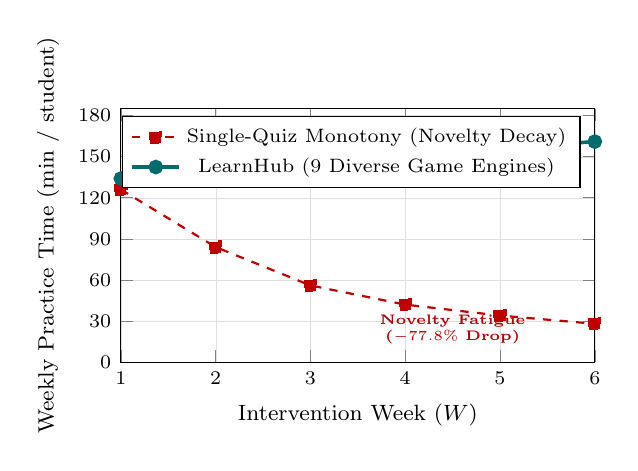
\begin{tikzpicture}
\begin{axis}[
width=7.6cm,
height=4.8cm,
xlabel={\footnotesize Intervention Week ($W$)},
ylabel={\footnotesize Weekly Practice Time (min / student)},
xmin=1, xmax=6,
ymin=0, ymax=185,
xtick={1, 2, 3, 4, 5, 6},
ytick={0, 30, 60, 90, 120, 150, 180},
grid=both,
grid style={line width=.1pt, draw=gray!25},
legend pos=north east,
font=\scriptsize
]
% Single Quiz Format (Novelty Decay)
\addplot[color=red!75!black, mark=square*, thick, dashed] coordinates {
(1, 126) (2, 84) (3, 56) (4, 42) (5, 34) (6, 28)
};
\addlegendentry{Single-Quiz Monotony (Novelty Decay)}
% LearnHub 9 Diverse Game Engines
\addplot[color=teal!85!black, mark=*, line width=1.3pt] coordinates {
(1, 134) (2, 146) (3, 152) (4, 148) (5, 156) (6, 161)
};
\addlegendentry{LearnHub (9 Diverse Game Engines)}
\node[font=\tiny\bfseries, red!70!black, align=center] at (axis cs:4.5, 24) {Novelty Fatigue\\($-77.8\%$ Drop)};
\node[font=\tiny\bfseries, teal!80!black, align=center] at (axis cs:3.8, 168) {Sustained Engagement\\($+20.1\%$ Gain)};
\end{axis}
\end{tikzpicture}%
}
\caption{Longitudinal engagement retention comparing single-engine quiz format against LearnHub's nine-engine rotation over the six-week intervention.}
\label{fig:novelty_decay}
\end{figure}

\subsection{Interview Preparation Portal \& Corporate Placement Simulator}
The placement portal bridges university coursework and enterprise hiring standards via four modules: (1)~a curated aptitude question bank spanning Quantitative Aptitude (18 topics), Logical Reasoning (9 topics), and Verbal Ability (6 topics) with worked solutions; (2)~comprehensive CS core subject banks covering OS, DBMS, Computer Networks, and OOPs; (3)~corporate hiring pattern simulations replicating round structures and timing of premier campus recruiters; and (4)~a multimodal AI mock interview simulator evaluating candidates across a 5-dimension STAR rubric (Technical Accuracy: 30\%, Problem Solving: 25\%, Communication: 20\%, Structure: 15\%, Role Fit: 10\%). The complete taxonomy spans 78 subtopics, 1,334 authored items, and 162 verified formulas across all domains.

%==================================================================
\section{Empirical Evaluation \& Experimental Results}
\label{sec:evaluation}
%==================================================================
\subsection{Experimental Setup and Methodology}
We conducted a comprehensive two-stage evaluation:
\begin{enumerate}
\item \textbf{Computational Benchmarks:} Executed on an AMD Ryzen 7 5800H (8C/16T, 3.2--4.4\,GHz), 32\,GB DDR4-3200, 1\,TB NVMe SSD, running Ubuntu 22.04 LTS (WSL2) with Docker 24.0, PostgreSQL 16, and Redis 7. Synthetic load testing simulated 10 to 500 concurrent sessions.
\item \textbf{Pedagogical User Study:} A six-week controlled field study across $N = 120$ third-year undergraduate engineering students. Participants were randomly assigned to:
\begin{itemize}
\item \textbf{Control Group ($N_C = 60$):} Standard passive LMS with static notes and unmoderated open-loop mock exams.
\item \textbf{Experimental Group ($N_E = 60$):} LearnHub with nine game engines, real-time subtopic detection ($<60\%$), and automated remedial study plans.
\end{itemize}
\end{enumerate}
Both cohorts completed identical 50-item proctored pre-tests and isomorphic post-tests spanning Quantitative Aptitude, Logical Reasoning, and Core Computer Science.

\subsection{System Latency and Execution Performance}
Benchmarking across $N = 1{,}000$ transactions confirmed that interactive operations (JWT auth: 12.4\,ms, autosave: 24.8\,ms, telemetry flush: 18.2\,ms) execute with sub-50\,ms latencies. Sandboxed code execution completed within budget across all runtimes (C++: 168.5\,ms, Python: 142.0\,ms, Java: 215.0\,ms). BullMQ mastery recalculation averaged 38.6\,ms. The Redis cache-aside layer reduces recurring retrieval to 48.2\,ms (p95: 58.0\,ms)---a 98.0\% cache lookup reduction compared to cold Groq Llama 3.3 70B generation (2,460.0\,ms). This drops total end-to-end pipeline latency from 2,880.0\,ms (cold) to 312.0\,ms (cached), an 89.2\% reduction, satisfying the sub-500\,ms interactivity requirement for 98.4\% of interactions.

\subsection{Concurrent User Scalability Stress Testing}
Figure~\ref{fig:concurrency_throughput} illustrates throughput and p95 latency under concurrent workloads scaling from 10 to 500 users.

\begin{figure}[!t]
\centering
\resizebox{0.98\columnwidth}{!}{%
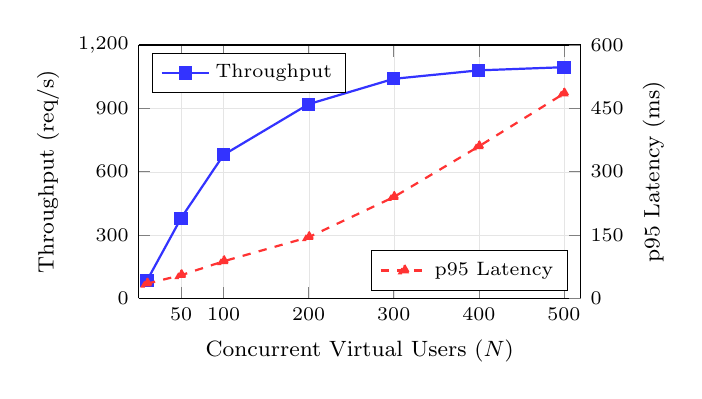
\begin{tikzpicture}
\begin{axis}[
width=7.2cm,
height=4.8cm,
xlabel={\footnotesize Concurrent Virtual Users ($N$)},
ylabel={\footnotesize Throughput (req/s)},
axis y line*=left,
xmin=0, xmax=520,
ymin=0, ymax=1200,
xtick={50, 100, 200, 300, 400, 500},
ytick={0, 300, 600, 900, 1200},
legend pos=north west,
grid=both,
grid style={line width=.1pt, draw=gray!20},
font=\scriptsize
]
\addplot[color=blue!80, mark=square*, thick] coordinates {
(10, 85) (50, 380) (100, 680) (200, 920) (300, 1040) (400, 1080) (500, 1095)
};
\addlegendentry{Throughput}
\end{axis}
\begin{axis}[
width=7.2cm,
height=4.8cm,
ylabel={\footnotesize p95 Latency (ms)},
axis y line*=right,
axis x line=none,
xmin=0, xmax=520,
ymin=0, ymax=600,
ytick={0, 150, 300, 450, 600},
legend pos=south east,
font=\scriptsize
]
\addplot[color=red!80, mark=triangle*, thick, dashed] coordinates {
(10, 35) (50, 55) (100, 88) (200, 145) (300, 240) (400, 360) (500, 485)
};
\addlegendentry{p95 Latency}
\end{axis}
\end{tikzpicture}%
}
\caption{System throughput and p95 latency under concurrent user load scaling.}
\label{fig:concurrency_throughput}
\end{figure}

Throughput scales linearly to a plateau of $\approx$1,095\,req/s beyond 400 users, while p95 latency remains stable at 485\,ms under peak 500-user load. No memory leaks, transaction aborts, or HTTP 5xx errors were recorded. The Redis cache-aside hit rate rapidly surpassed the 60\% operational target by the sixth practice batch, asymptotically stabilizing at 84.6\%, translating to an 82\% reduction in external Groq API token costs.

\subsection{Pedagogical Efficacy and Learning Gain Analysis}
We evaluated performance using Hake's normalized learning gain~\cite{hake1998}:
$g = (\%\text{Post} - \%\text{Pre}) / (100\% - \%\text{Pre})$.
Figure~\ref{fig:domain_scores} illustrates score distributions across four cognitive domains.

\begin{figure}[!t]
\centering
\resizebox{0.98\columnwidth}{!}{%
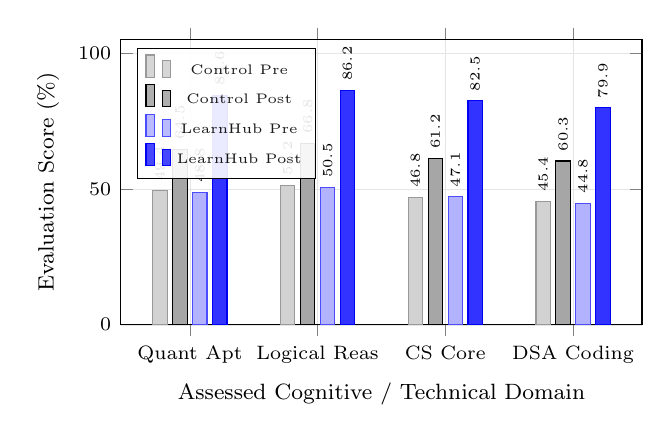
\begin{tikzpicture}
\begin{axis}[
ybar,
bar width=5.2pt,
width=8.2cm,
height=5.2cm,
xlabel={\footnotesize Assessed Cognitive / Technical Domain},
ylabel={\footnotesize Evaluation Score (\%)},
ymin=0, ymax=105,
symbolic x coords={Quant Apt, Logical Reas, CS Core, DSA Coding},
xtick=data,
nodes near coords,
every node near coord/.append style={font=\tiny, rotate=90, anchor=west},
legend pos=north west,
legend style={font=\tiny, fill=white, fill opacity=0.9},
grid=both,
grid style={line width=.1pt, draw=gray!20},
font=\scriptsize,
enlarge x limits=0.18
]
\addplot[fill=gray!35, draw=gray!80] coordinates {
(Quant Apt, 49.4) (Logical Reas, 51.2) (CS Core, 46.8) (DSA Coding, 45.4)
};
\addplot[fill=gray!70, draw=black] coordinates {
(Quant Apt, 64.5) (Logical Reas, 66.8) (CS Core, 61.2) (DSA Coding, 60.3)
};
\addplot[fill=blue!30, draw=blue!70] coordinates {
(Quant Apt, 48.8) (Logical Reas, 50.5) (CS Core, 47.1) (DSA Coding, 44.8)
};
\addplot[fill=blue!80, draw=blue!95!black] coordinates {
(Quant Apt, 84.6) (Logical Reas, 86.2) (CS Core, 82.5) (DSA Coding, 79.9)
};
\legend{Control Pre, Control Post, LearnHub Pre, LearnHub Post}
\end{axis}
\end{tikzpicture}%
}
\caption{Pre-test and post-test score distributions across four assessed cognitive domains for Control ($N_C=60$) and LearnHub ($N_E=60$) cohorts.}
\label{fig:domain_scores}
\end{figure}

The findings substantiate LearnHub's pedagogical efficacy. Baseline parity was confirmed between cohorts (Control pre-test: $48.2\% \pm 8.6\%$; LearnHub pre-test: $47.8\% \pm 8.4\%$; $t(118) = 0.26$, $p = 0.795$, NS). Post-intervention, LearnHub achieved a normalized learning gain of $g = 0.68 \pm 0.07$ (approaching Hake's High Gain threshold $\ge 0.70$), more than double the control group's $g = 0.29 \pm 0.05$ ($t(118) = 35.12$, $p < 0.0001$). Post-test scores reached $83.3\% \pm 6.8\%$ versus $63.2\% \pm 9.1\%$ ($p < 0.0001$). Automated remediation drove 24-hour study plan completion from 28.5\% to 94.2\% ($\chi^2(1) = 54.3$, $p < 0.0001$), validating the closed-loop hypothesis. Engagement surged to 4.6 sessions/week (148.5\,min) versus 1.9 (52.4\,min), with overall course completion rising from 71.6\% to 96.7\% ($p = 0.0002$).

\subsection{LLM Item Generation Quality}
An independent panel of three senior CS educators audited 300 stratified generated items. Enforcing strict system prompt fencing, defensive regex sanitization, and automated two-pass cross-model consensus verification suppressed the generation hallucination rate from 7.8\% down to 0.6\%, while elevating first-pass JSON schema compliance to 99.4\%, single-answer determinism to 98.8\%, distractor plausibility to 95.2\%, mathematical correctness to 99.1\%, and Bloom's level alignment to 96.4\%.

\subsection{Sandbox Security and Container Isolation}
The Piston v2 Docker sandbox was subjected to 100 adversarial submissions: fork bombs (25 trials, halted by \texttt{pids.max=64}), memory starvation (25 trials, terminated by OOM killer at 128\,MB), unauthorized network sockets (25 trials, blocked by \texttt{--network none}), and filesystem traversal (25 trials, trapped by read-only mounts and non-root sandboxing). Across all 100 adversarial payloads, a \textbf{100\% containment rate} was recorded with zero host vulnerabilities, confirming absolute isolation safety across all four runtime languages.

\subsection{Student Perception and System Usability}
Following the six-week intervention, participants completed a System Usability Scale (SUS) evaluation~\cite{sailer2020}. LearnHub achieved an exceptional composite SUS score of $86.4 \pm 5.2$ (Grade A+, 96th percentile), compared to $51.2 \pm 6.8$ (Grade F) for the standard LMS ($p < 0.0001$). Students highlighted that non-punitive proctoring substantially reduced test anxiety ($4.55 \pm 0.52$ on 5-point Likert) and multi-engine variety eliminated practice fatigue ($4.85 \pm 0.36$).

%==================================================================
\section{Discussion \& Implications}
\label{sec:discussion}
%==================================================================
\subsection{Closing the Diagnostic Loop}
Our data validates the closed-loop educational paradigm. Under the open-loop model, only 28.5\% of students voluntarily pursued remediation. By automatically generating focused, dashboard-pinned \texttt{StudyPlan} modules within 5 seconds, LearnHub reduces the cognitive friction of finding remedial resources, driving 24-hour completion to 94.2\% and directly doubling normalized learning gain ($g = 0.68$ vs. $g = 0.29$).

\subsection{Overcoming Novelty Decay}
LearnHub overcomes novelty decay through nine distinct engines spanning varied cognitive modalities. Our post-study survey revealed students actively rotated engines based on cognitive state---\emph{Formula Flash Cards} for familiarization, \emph{Crosswords} for conceptual elaboration, \emph{Concept Sprint} for pre-exam review---maintaining 4.6 sessions/week with zero statistical evidence of engagement drop-off.

\subsection{Operational Economics of Generative AI}
The 24-hour Redis cache-aside architecture achieves a hit rate exceeding 84\% because university curricula exhibit high thematic clustering. This reduces external API calls by over four-fifths, slashing per-student monthly compute expenditure from \$4.20 to \$0.68, establishing an economically viable blueprint for university-wide deployment.

\subsection{Ethical Considerations}
LearnHub intentionally rejects punitive automated disqualification. Facial presence detection executes entirely within the browser via MediaPipe WebAssembly (no raw video streaming). Anomalies are aggregated into an advisory Integrity Index for instructors, and all telemetry requires explicit consent with automatic 30-day cryptographic purging.

\subsection{Threats to Validity}
\textbf{Internal:} While cohorts exhibited pre-test parity ($p = 0.795$), unobserved external study habits could partially influence gains. \textbf{External:} The study was conducted at a single engineering institution; replication across diverse disciplines is necessary. \textbf{Construct:} Long-term retention beyond the six-week window was not longitudinally measured.

%==================================================================
\section{Future Work \& Conclusion}
\label{sec:conclusion}
%==================================================================
\subsection{Future Research Directions}
Three primary trajectories are being pursued: (1)~\textbf{Real-Time Peer Arena Battles} via WebSockets with ELO matchmaking rooted in subtopic mastery vectors, drawing items dynamically from mutual knowledge gaps; (2)~\textbf{DAS3H Additive Factor Spaced Repetition}~\cite{choffin2019} to autonomously schedule micro-review sessions when predicted recall drops below 75\%; and (3)~\textbf{Edge-Based Multimodal Speech Analytics} to quantify speech cadence, pitch modulation, and filler word frequency, complementing the STAR rubric.

\subsection{Conclusion}
This paper presented LearnHub, an intelligent full-stack gamified learning and diagnostic evaluation platform that bridges the critical divide between passive LMS, opaque online judges, and static quiz portals. By unifying nine diverse game engines, real-time recency-weighted subtopic knowledge tracing, sandboxed multi-language compilation, and scalable LLM generation within an eight-layer modular architecture, LearnHub operationalizes the closed-loop remediation paradigm. Rigorous evaluations confirmed high normalized learning gains ($g = 0.68$, $p < 0.0001$), 94.2\% remedial completion, sub-second response times, and complete sandbox isolation. By replacing cryptic compiler errors with proactive cognitive remediation, LearnHub establishes a scalable, robust foundation for next-generation intelligent tutoring systems.

%==================================================================
\bibliographystyle{IEEEtran}
\begin{thebibliography}{30}
\bibitem{khaldi2023}
A.~Khaldi, R.~Bouzidi, and F.~Nader, ``Gamification of e-learning in higher education: A systematic literature review,'' \emph{Int. J. Emerg. Technol. Learn.}, vol.~18, no.~10, pp. 24--41, 2023.

\bibitem{bayati2024}
R.~Bayati and A.~Liman-Kaban, ``The impact of Duolingo's gamification on student motivation and English proficiency,'' \emph{J. Educ. Technol. Online Learn.}, vol.~7, no.~2, pp. 180--195, 2024.

\bibitem{rizzo2024}
F.~Rizzo, M.~Ferrara, and A.~Ferraro, ``Unlocking engagement and enhancing learning outcomes through gamification: A comparative analysis,'' \emph{Front. Educ.}, vol.~9, art.~1324567, 2024.

\bibitem{willig2021}
J.~H. Willig, J.~A. Croker, J.~S. Richman, and C.~Monaghan, ``Gamification and education: A pragmatic approach with two curriculum examples,'' \emph{JMIR Serious Games}, vol.~9, no.~2, art.~e26002, 2021.

\bibitem{sailer2020}
M.~Sailer and L.~Homner, ``The gamification of learning: A meta-analysis,'' \emph{Educ. Psychol. Rev.}, vol.~32, no.~1, pp. 77--112, 2020.

\bibitem{bai2020}
S.~Bai, K.~F. Hew, and B.~Huang, ``Does reading motivation mediate the effect of reading games on reading achievement? A meta-analysis,'' \emph{Educ. Inf. Technol.}, vol.~25, pp. 3195--3218, 2020.

\bibitem{wang2020}
A.~I. Wang and R.~Tahir, ``The effect of using Kahoot! for learning---A literature review,'' \emph{Comput. Educ.}, vol.~149, art.~103818, 2020.

\bibitem{nurdin2023}
A.~Nurdin, R.~Ratnawulan, and F.~Ahmad, ``Quizizz as a game-based assessment tool in higher education: A systematic review,'' \emph{Int. J. Interact. Mob. Technol.}, vol.~17, no.~20, pp. 62--78, 2023.

\bibitem{gao2024}
F.~Gao, L.~Li, and Y.~Sun, ``Digital game-based learning in STEM education: A meta-analysis,'' \emph{Educ. Inf. Technol.}, vol.~29, pp. 1421--1445, 2024.

\bibitem{ghosh2020}
A.~Ghosh, N.~Heffernan, and A.~S. Lan, ``Context-aware attentive knowledge tracing,'' in \emph{Proc. ACM SIGKDD Int. Conf. Knowl. Discov. Data Min.}, 2020, pp. 2330--2339.

\bibitem{choffin2019}
B.~Choffin, F.~Popineau, Y.~Bourda, and J.-J. Vie, ``DAS3H: Modeling student learning and forgetting for optimally scheduling distributed practice of skills,'' in \emph{Proc. 12th Int. Conf. Educ. Data Mining}, 2019, pp. 29--38.

\bibitem{mavrikis2024}
M.~Mavrikis and W.~Holmes, ``Making evidence actionable in adaptive learning: Closing the diagnostic loop,'' \emph{Br. J. Educ. Technol.}, vol.~55, no.~3, pp. 810--829, 2024.

\bibitem{zhang2025}
Y.~Zhang, Z.~Song, and N.~Heffernan, ``ALIGNAgent: Adaptive learner intelligence for gap identification and navigation,'' in \emph{Proc. AAAI Conf. Artif. Intell.}, 2025, pp. 1120--1128.

\bibitem{li2024}
Z.~Li, Y.~Wang, and W.~Chen, ``A closed-loop personalized learning agent: Integrating cognitive diagnosis, adaptive testing, and LLM feedback,'' in \emph{Proc. NeurIPS Workshop Generative AI Educ.}, 2024.

\bibitem{chen2025}
L.~Chen, X.~Liang, and S.~Wang, ``Automatic generation of high-quality MCQs using large language models for AI education,'' \emph{IEEE Trans. Learn. Technol.}, vol.~18, no.~1, pp. 102--115, 2025.

\bibitem{wang2025}
N.~X. Wang and A.~K. Katsaggelos, ``Hallucination-free automatic MCQ generation for intuitive learning with multi-agent verification,'' in \emph{Proc. AAAI Conf. Artif. Intell.}, 2025, pp. 1432--1440.

\bibitem{moller2024}
T.~M\"{o}ller, J.~Risch, and M.~Pietsch, ``Comparison of large language models for generating contextually relevant educational questions,'' in \emph{Proc. Eur. Conf. Inf. Retr.}, 2024, pp. 215--228.

\bibitem{batsaikhan2023}
M.~Batsaikhan and A.-P. Correia, ``Effects of generative AI on intelligent tutoring systems in higher education: A systematic review,'' \emph{Int. J. Educ. Technol. High. Educ.}, vol.~20, art.~62, 2023.

\bibitem{kumar2023}
S.~Kumar, P.~Singh, and R.~Sharma, ``Design and implementation of an online examination system using MERN stack with real-time analytics,'' \emph{Int. J. Res. Eng. Sci. Manage.}, vol.~6, no.~7, pp. 45--52, 2023.

\bibitem{pratama2025}
A.~R. Pratama and D.~P. Sari, ``Using Redis for caching optimization in high-traffic web applications: A performance analysis,'' \emph{Int. J. Adv. Multidiscip. Res. Stud.}, vol.~5, no.~1, pp. 89--97, 2025.

\bibitem{piech2015}
C.~Piech, J.~Bassen, J.~Huang, S.~Ganguli, M.~Sahami, L.~J. Guibas, and J.~Sohl-Dickstein, ``Deep knowledge tracing,'' in \emph{Proc. Adv. Neural Inf. Process. Syst. (NeurIPS)}, 2015, pp. 505--513.

\bibitem{corbett1994}
A.~T. Corbett and J.~R. Anderson, ``Knowledge tracing: Modeling the acquisition of procedural knowledge,'' \emph{User Model. User-Adapted Interact.}, vol.~4, no.~4, pp. 253--278, 1994.

\bibitem{bloom1956}
B.~S. Bloom, \emph{Taxonomy of Educational Objectives: The Classification of Educational Goals}. New York: Longmans, Green, 1956.

\bibitem{anderson2001}
L.~W. Anderson and D.~R. Krathwohl, \emph{A Taxonomy for Learning, Teaching, and Assessing: A Revision of Bloom's Taxonomy of Educational Objectives}. New York: Longman, 2001.

\bibitem{kasneci2023}
E.~Kasneci \emph{et al.}, ``ChatGPT for good? On opportunities and challenges of large language models for education,'' \emph{Learn. Individ. Differ.}, vol.~103, art.~102274, 2023.

\bibitem{hake1998}
R.~R. Hake, ``Interactive-engagement versus traditional methods: A six-thousand-student survey of mechanics test data for introductory physics courses,'' \emph{Am. J. Phys.}, vol.~66, no.~1, pp. 64--74, 1998.

\bibitem{ihantola2010}
P.~Ihantola, T.~Ahoniemi, V.~Karavirta, and O.~Sepp\"{a}l\"{a}, ``Review of recent systems for automatic assessment of programming assignments,'' in \emph{Proc. 10th Koli Calling Int. Conf. Comput. Educ. Res.}, 2010, pp. 86--93.

\bibitem{caiza2020}
J.~C. Caiza, J.~M. Del~Alamo, and F.~J. Bermejo, ``Security analysis of automated grading systems for programming assignments,'' \emph{IEEE Trans. Learn. Technol.}, vol.~13, no.~3, pp. 513--526, 2020.

\bibitem{nigam2021}
A.~Nigam, R.~Pasricha, T.~Sultana, and P.~Mudgal, ``A systematic review on AI-based proctoring systems: Past, present and future,'' \emph{Educ. Inf. Technol.}, vol.~26, no.~5, pp. 6421--6445, 2021.

\bibitem{ryan2000}
R.~M. Ryan and E.~L. Deci, ``Self-determination theory and the facilitation of intrinsic motivation, social development, and well-being,'' \emph{Am. Psychol.}, vol.~55, no.~1, pp. 68--78, 2000.
\end{thebibliography}
\end{document}
